\section{Estimating Speciation \& Extinction Rates Through Time}

\subsection{Outline}

This tutorial describes how to specify an episodic branching-process models in \RevBayes;
a birth-death process where diversification rates vary episodically through time model by piecewise constant rates \citep{Stadler2011,Hoehna2015a}.
The probabilistic graphical model is given for each component of this tutorial.
Finally, you will estimate speciation and extinction rates through-time using Markov chain Monte Carlo (MCMC).


\subsection{Requirements}
We assume that you have read and hopefully completed the following tutorials:
\begin{itemize}
\item RB\_Getting\_Started
\item RB\_Basics\_Tutorial
\item RB\_BayesFactor\_Tutorial
\item RB\_BasicDiversificationRate\_Tutorial
\end{itemize}
Note that the RB\_Basics\_Tutorial introduces the basic syntax of \Rev but does not cover any phylogenetic models.
You may skip the RB\_Basics\_Tutorial if you have some familiarity with \R.
The RB\_BayesFactor\_Tutorial introduced Bayesian model selection by means of Bayes factors, which can be skipped by readers familiar with Bayesian model selection.
We tried to keep this tutorial very basic and introduce all the language concepts and theory on the way.
You may only need the RB\_Basics\_Tutorial for a more in-depth discussion of concepts in \Rev.


%%%%%%%%
%%   Data   %%
%%%%%%%%
\section{Data and files}

We provide the data file(s) which we will use in this tutorial.
You may want to use your own data instead.
In the \cl{data} folder, you will find the following files
\begin{itemize}
\item \cl{primates\_springer.tre}: Dated primates phylogeny including 369 out of 450 species from \cite{Springer2012}.
\end{itemize}


\impmark{Open the tree \cl{data/primates\_springer.tre} in FigTree.}


\bigskip
\section{Episodic Birth-Death Model}

The basic idea behind the model is that speciation and extinction rates are piecewise constant but can be different for different time intervals.
Thus, we will divide time into equal time interval with the only exception that the first 20\% of the time do not have any rate changes.
Our only reason to do so is because there are two few lineages in the reconstructed tree at that time to obtain reliable parameter estimates.
An overview of the underlying theory of the specific model and implementation is given in \citep{Hoehna2015a}.

We assume that the log-transformed rates are drawn from a normal distribution.
Furthermore, we will assume that rates are autocorrelated, that is, rates in the next time interval will be centered around the rates in the current time interval.
The assumption of autocorrelated rates does not only makes sense biologically but also improves our ability to estimate parameters.
\begin{figure}[h!]
\centering
\fbox{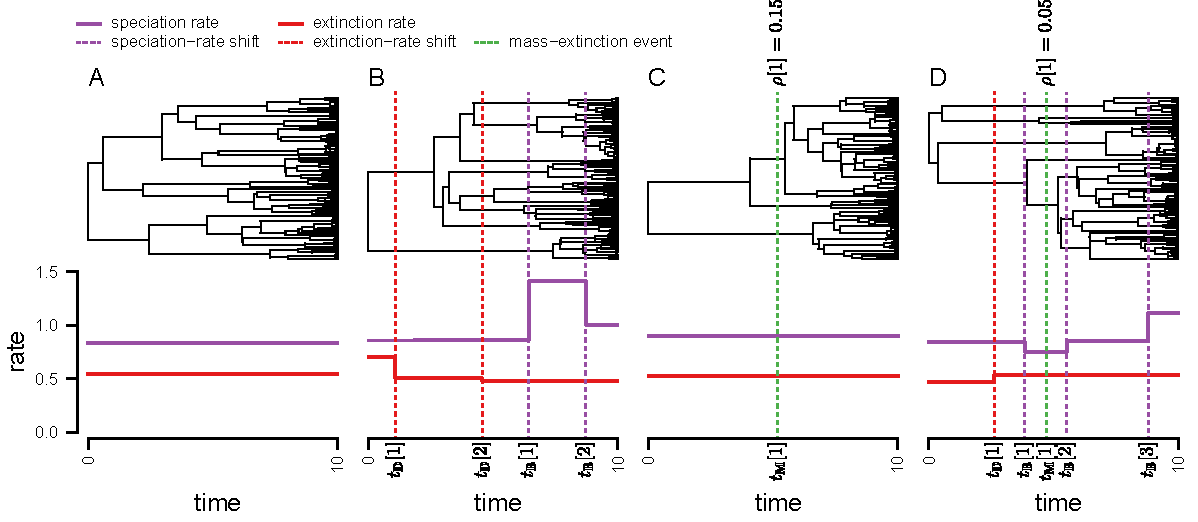
\includegraphics[width=\textwidth]{\ResourcePath figures/EBD_scenarios.pdf}}
\caption{\small Four scenarios of birth-death models.}
\label{fig:EBD}
\end{figure}



\subsection{Read the tree}

Begin by reading in the observed tree. 

{\tt \begin{snugshade*}
\begin{lstlisting}
T <- readTrees("data/primates_springer.tre")[1]
\end{lstlisting}
\end{snugshade*}}

From this tree, we can get some helpful variables:
{\tt \begin{snugshade*}
\begin{lstlisting}
taxa <- T.taxa()
\end{lstlisting}
\end{snugshade*}}

Additionally, we can initialize an iterator variable for our vector of moves:
{\tt \begin{snugshade*}
\begin{lstlisting}
mvi = 0
\end{lstlisting}
\end{snugshade*}}

Finally, we create a helper variable that specifies the number of intervals.
{\tt \begin{snugshade*}
\begin{lstlisting}
NUM_INTERVALS = 10
\end{lstlisting}
\end{snugshade*}}
Using this variable we can easily change our script to break-up time into many or few intervals.



\subsection{Specifying the model}

\subsubsection{Priors on rates}
We start by specifying prior distributions on the rates.
Each interval specific speciation and extinction rate will be drawn from a normal distribution.
Thus, we a parameter for the standard deviation of those normal distributions.
We use an exponential hyperprior with rate 1.0 to estimate the standard deviation, but assume that all speciation rates and all extinction rates share the same standard deviation.
The motivation for an exponential hyperprior is that it has the highest probability density at 0 which would make he variance between rates 0 too and thus represent a constant rate process.
The data will tell us if there should be much variation in rates through time.
{\tt \begin{snugshade*}
\begin{lstlisting}
speciation_sd ~ dnExponential(1.0)
extinction_sd ~ dnExponential(1.0)
\end{lstlisting}
\end{snugshade*}}
We apply a simple scaling move on each prior parameter.
{\tt \begin{snugshade*}
\begin{lstlisting}
moves[++mvi] = mvScale(speciation_sd,weight=5.0)
moves[++mvi] = mvScale(extinction_sd,weight=5.0)
\end{lstlisting}
\end{snugshade*}}

The second prior parameter that we need to specify is mean of the speciation and extinction rate at present.
This is because we are actually modeling rate-changes backwards in time and there is no previous rate for the rate at the present.
Thus we use a uniform distribution between -5 and 5 because of lack of prior knowledge.
{\tt \begin{snugshade*}
\begin{lstlisting}
# draw the mean from a uniform distribution
speciation_prior_mean ~ dnUniform(-5.0,5.0)
extinction_prior_mean ~ dnUniform(-5.0,5.0)
\end{lstlisting}
\end{snugshade*}}
This time we will apply a simple sliding window move because both parameters are location parameters instead of scale or variance parameters.
{\tt \begin{snugshade*}
\begin{lstlisting}
moves[++mvi] = mvSlide(speciation_prior_mean,weight=5.0)
moves[++mvi] = mvSlide(extinction_prior_mean,weight=5.0)
\end{lstlisting}
\end{snugshade*}}


\subsubsection{Specifying episodic rates}
As we mentioned before, we will apply normal distributions as priors for each rate.
We begin with the rate at the present.
The rates at the present will be specified slightly differently because they are not correlated to any previous rates.
Note that we store the variables in vectors.
{\tt \begin{snugshade*}
\begin{lstlisting}
log_speciation[1] ~ dnNormal( mean=speciation_prior_mean, sd=speciation_sd )
log_extinction[1] ~ dnNormal( mean=extinction_prior_mean, sd=extinction_sd )
\end{lstlisting}
\end{snugshade*}}
Again, we apply simple sliding window moves for the rates.
Normally we would use scaling moves but in this case we work on the log-transformed parameters and thus sliding moves perform better.
If you are keen you can test the differences.
{\tt \begin{snugshade*}
\begin{lstlisting}
moves[++mvi] = mvSlide(log_speciation[1], weight=2)
moves[++mvi] = mvSlide(log_extinction[1], weight=2)
\end{lstlisting}
\end{snugshade*}}
Now we transform the parameters.
{\tt \begin{snugshade*}
\begin{lstlisting}
speciation[1] := exp( log_speciation[1] )
extinction[1] := exp( log_extinction[1] )
\end{lstlisting}
\end{snugshade*}}

Then we repeat the specification for the speciation and extinction rates for each time interval.
This can be done efficiently using a \cl{for}-loop.
We will use a specific index variable so that we can easier refer to the rate at the previous interval.
{\tt \begin{snugshade*}
\begin{lstlisting}
for (i in 1:NUM_INTERVALS) {
    index = i+1
    
    log_speciation[index] ~ dnNormal( mean=log_speciation[i], sd=speciation_sd )
    log_extinction[index] ~ dnNormal( mean=log_extinction[i], sd=extinction_sd )

    moves[++mvi] = mvSlide(log_speciation[index], weight=2)
    moves[++mvi] = mvSlide(log_extinction[index], weight=2)

    speciation[index] := exp( log_speciation[index] )
    extinction[index] := exp( log_extinction[index] )

}
\end{lstlisting}
\end{snugshade*}}
Finally, we apply moves that slide all values in the vectors, \IE all speciation or extinction rates, by the same amount. 
This again considerably improves the efficiency of our MCMC analysis.
{\tt \begin{snugshade*}
\begin{lstlisting}
moves[++mvi] = mvVectorSlide(log_speciation, weight=10)
moves[++mvi] = mvVectorSlide(log_extinction, weight=10)
\end{lstlisting}
\end{snugshade*}}


\subsubsection{Setting up the time inverals}
In \RevBayes you actually have the possibility unequal time intervals or even different intervals for the speciation and extinction rate.
This is achieved by providing a vector of times when each interval ends.
Here we simply break-up the most recent 80\% of time since the root in equal intervals.
{\tt \begin{snugshade*}
\begin{lstlisting}
interval_times = T.rootAge() * (1:NUM_INTERVALS) / (NUM_INTERVALS) * 0.8
\end{lstlisting}
\end{snugshade*}}


\subsubsection{Incomplete Taxon Sampling}

We know that we have sampled 367 out of 450 living primate species. 
To account for this we can set the sampling parameter as a constant node with a value of 369/450
{\tt \begin{snugshade*}
\begin{lstlisting}
rho <- T.ntips()/450
\end{lstlisting}
\end{snugshade*}}


\subsubsection{Root age}

The birth-death process requires a parameter for the root age.
In this exercise we use a fix tree and thus we know the age of the tree.
Hence, we can get the value for the root from the \citet{Springer2012} tree.
{\tt \begin{snugshade*}
\begin{lstlisting}
root_time <- T.rootAge()
\end{lstlisting}
\end{snugshade*}}

\subsubsection{The time tree}

Now we have all of the parameters we need to specify the full episodic birth-death model. 
We initialize the stochastic node representing the time tree.
{\tt \begin{snugshade*}
\begin{lstlisting}
timetree ~ dnEpisodicBirthDeath(rootAge=T.rootAge(), lambdaRates=speciation, lambdaTimes=interval_times, muRates=extinction, muTimes=interval_times, rho=rho, taxa=taxa)
\end{lstlisting}
\end{snugshade*}}
And then we attach data to it.
{\tt \begin{snugshade*}
\begin{lstlisting}
timetree.clamp(T)
\end{lstlisting}
\end{snugshade*}}

Finally, we create a workspace object of our whole model using the \cl{model()} function. 
{\tt \begin{snugshade*}
\begin{lstlisting}
mymodel = model(speciation)
\end{lstlisting}
\end{snugshade*}}

The \cl{model()} function traversed all of the connections and found all of the nodes we specified. 


\subsection{Running an MCMC analysis}

\subsubsection{Specifying Monitors}

For our MCMC analysis, we need to set up a vector of \textit{monitors} to record the states of our Markov chain. 
First, we will initialize the model monitor using the \cl{mnModel} function. This creates a new monitor variable that will output the states for all model parameters when passed into a MCMC function. 
{\tt \begin{snugshade*}
\begin{lstlisting}
monitors[1] = mnModel(filename="output/primates_BSBD.log",printgen=10, separator = TAB)
\end{lstlisting}
\end{snugshade*}}

Additionally, we create two separate file monitors, one for each vector of speciation and extinction rates.
We want to have the speciation and extinction rates stored separately so that we can plot them nicely afterwards.
{\tt \begin{snugshade*}
\begin{lstlisting}
monitors[2] = mnFile(filename="output/primates_EBD_speciation.log",printgen=10, separator = TAB, speciation)
monitors[3] = mnFile(filename="output/primates_EBD_extinction.log",printgen=10, separator = TAB, extinction)
\end{lstlisting}
\end{snugshade*}}

Finally, create a screen monitor that will report the states of specified variables to the screen with \cl{mnScreen}:
{\tt \begin{snugshade*}
\begin{lstlisting}
monitors[4] = mnScreen(printgen=1000, speciation)
\end{lstlisting}
\end{snugshade*}}

\subsubsection{Initializing and Running the MCMC Simulation}

With a fully specified model, a set of monitors, and a set of moves, we can now set up the MCMC algorithm that will sample parameter values in proportion to their posterior probability. The \cl{mcmc()} function will create our MCMC object:
{\tt \begin{snugshade*}
\begin{lstlisting}
mymcmc = mcmc(mymodel, monitors, moves)
\end{lstlisting}
\end{snugshade*}}

First, we will run a pre-burnin to tune the moves and to obtain starting values from the posterior distribution.
{\tt \begin{snugshade*}
\begin{lstlisting}
mymcmc.burnin(generations=10000,tuningInterval=200)
\end{lstlisting}
\end{snugshade*}}


Now, run the MCMC:
{\tt \begin{snugshade*}
\begin{lstlisting}
mymcmc.run(generations=50000)
\end{lstlisting}
\end{snugshade*}}

When the analysis is complete, you will have the monitored files in your output directory.
You can then visualize the rates through time using \R.
We have provided a very simple example script for you.
Just start \R in the main directory for this analysis and then type the following commands:
{\tt \begin{snugshade*}
\begin{lstlisting}
source("RevBayes_scripts/Plot_EBD_RevBayes.R")
plot.EBD("output/primates_EBD","Episodic_Rates")
\end{lstlisting}
\end{snugshade*}}

\impmark{The \Rev file for performing this analysis: \href{https://github.com/revbayes/revbayes_tutorial/raw/master/RB_DiversificationRateEpisodic_Tutorial/RevBayes_scripts/mcmc_EBD.Rev}{\cl{mcmc\_EBD.Rev}}.}
\impmark{An \R file for plotting the output: \href{https://github.com/revbayes/revbayes_tutorial/raw/master/RB_DiversificationRateEpisodic_Tutorial/RevBayes_scripts/Plot_EBD_RevBayes.R}{\cl{Plot\_EBD\_RevBayes.R}}.}


\subsection{Exercise}

\begin{itemize}
\item Run an MCMC simulation to estimate the posterior distribution of the speciation rate and extinction rate.
\item Visualize the rate through time using \R.
\item Do you see evidence for rate decreases or increases? What is the general trend?
\item Run the analysis using a different number of intervals, \EG 5 or 50. How do the rates change?
\item Modify the model by specifying a prior on the log-diversification and log-turnover rate and then estimate the diversification rates through time. Do you see any differences in the estimates? 
\end{itemize}




\bibliographystyle{sysbio}
\bibliography{\GlobalResourcePath refs}
